\section{Семинар 1.04.26}

% @startuml
% left to right direction

% rectangle "Внешний мир" as EXT
% rectangle "Рынок товаров и услуг" as GOODS
% rectangle "Фирмы" as FIRM
% rectangle "Рынок факторов производства" as FACTORS
% rectangle "Домохозяйства" as HOUSE
% rectangle "Финансовый рынок" as FIN
% rectangle "Государство" as GOV

% ' Внешний сектор
% GOODS --> EXT : Импорт (Im)
% EXT --> GOODS : Экспорт (Ex)

% note right of EXT
% Чистый экспорт:
% Xn = Ex - Im
% end note

% ' Рынок товаров и услуг
% GOODS --> FIRM : Совокупные расходы (AE)

% note right of GOODS
% AE = C + I + G + Xn
% ВВП по расходам
% end note

% ' Фирмы и рынок факторов
% FIRM --> FACTORS : Доходы факторов (Y)

% note right of FACTORS
% Y = ВВП по доходам
% Y = C + S + T
% end note

% ' Домохозяйства
% FACTORS --> HOUSE : Располагаемый доход (Yd)

% note right of HOUSE
% Yd = Y - T
% Yd = C + S
% end note

% HOUSE --> GOODS : Потребление (C)
% HOUSE --> FIN : Сбережения (S)
% HOUSE --> GOV : Налоги (Tx)

% ' Финансовый рынок
% FIN --> FIRM : Инвестиции (I)

% ' Государство
% GOV --> GOODS : Госрасходы (G)
% GOV --> HOUSE : Трансферты (Tr)
% FIRM --> GOV : Налоги (Tx)

% note bottom of GOV
% Чистые налоги:
% T = Tx - Tr
% end note

% @enduml

\begin{figure}[h]
  \centering
  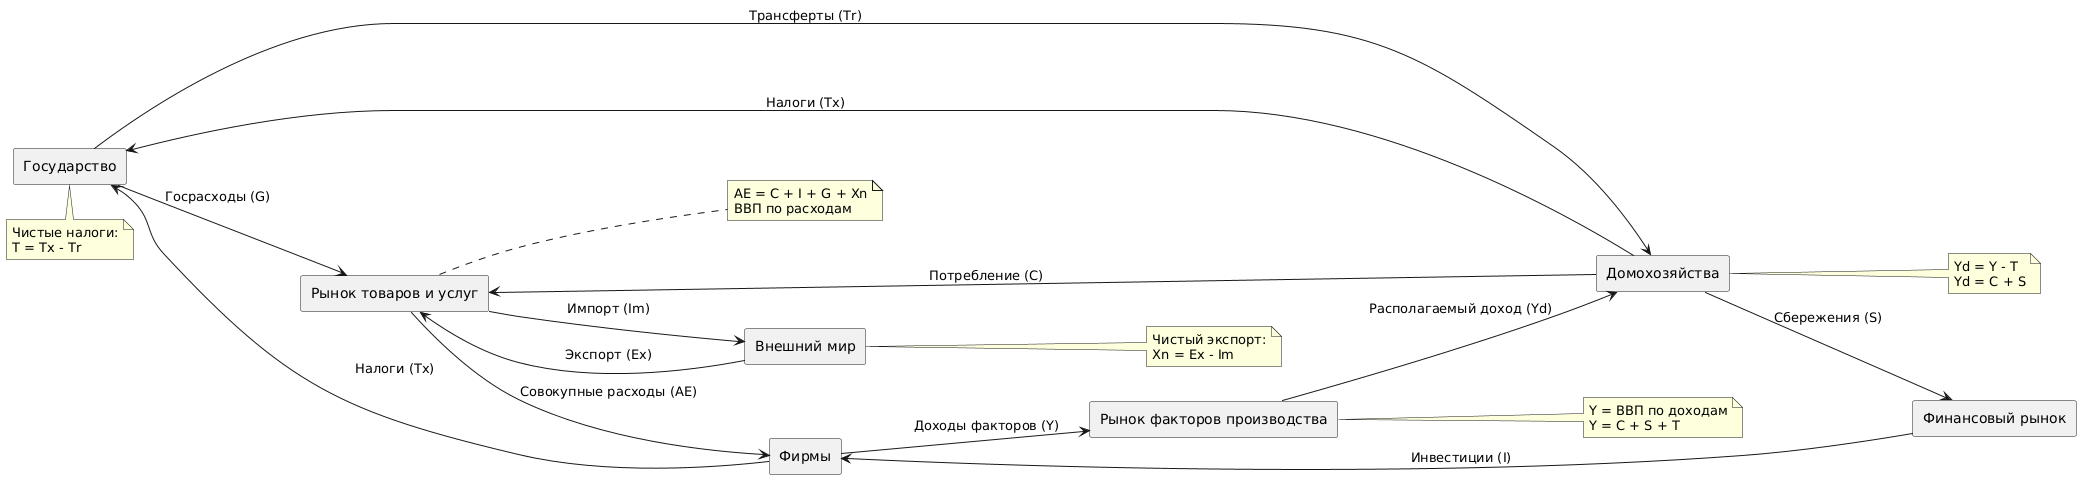
\includegraphics[width=1\textwidth]{tickets/files/Circular_Flow_Economy.png}
  \caption{Круговорот ресурсов и благ в экономике}
  \label{fig:10426120338.png}
\end{figure}

\begin{theorem}[Основное макроэкономическое тождество]
\[
  AE = Y
\]
\[
  AE = C + I + G + X_n
\]
\[
  Y = C + S + T
\]
\[
  X_n = Ex - Im,\quad T = Tx - Tr
\]
\end{theorem}

\paragraph{Инъекции и утечки}
В открытой экономике с государством равновесие можно записать как
\[
  I + G + Ex + Tr = S + Tx + Im
\]
\textbf{Инъекции (injections):} добавляют расходы/доход в круговорот.
\begin{itemize}
  \item $I$ --- инвестиции фирм.
  \item $G$ --- государственные закупки товаров и услуг.
  \item $Ex$ --- экспорт (внешний спрос на отечественные товары).
  \item $Tr$ --- трансферты от государства домохозяйствам.
\end{itemize}
\textbf{Утечки (leakages):} выводят средства из круговорота.
\begin{itemize}
  \item $S$ --- сбережения домохозяйств.
  \item $Tx$ --- налоги (выплаты государству).
  \item $Im$ --- импорт (расходы на зарубежные товары).
\end{itemize}
Эквивалентная запись через чистые налоги и чистый экспорт:
\[
  I + G + X_n = S + T
\]
